\documentclass[a4paper,12pt]{article}
\usepackage{tikz}
\usetikzlibrary{circuits.logic.US, positioning}
\usepackage[utf8]{inputenc}
\usepackage{amsmath}
\usepackage{geometry}
\geometry{margin=1in}
\usepackage{caption}
\usepackage{subcaption}
\usepackage{xcolor}
\usepackage{fancyhdr}
\usepackage{array}
\usepackage{float}
\usepackage{enumitem}
\definecolor{darkskyblue}{rgb}{0.0, 0.5, 1.0}
\definecolor{skyblue}{RGB}{135, 206, 235}

\geometry{a4paper, top=0.7in, left=1in, right=1in, bottom=1in}

\begin{document}
\pagestyle{empty} % Start with empty page style

\thispagestyle{fancy} % Apply fancy style only to the first page
\fancyhf{} % Clear header and footer
\renewcommand{\headrulewidth}{0pt} % Remove header rule

\fancyhead[L]{% Left header
    
\includegraphics[width=6.5cm, height=1.3cm]{img3.png}
}

\fancyhead[R]{% Right header
    Name: K.Saisusmitha \\
    Batch: COMETFWC018 \\
    Date: 16 May 2025
}

\vspace{1.5cm}
\begin{center}
    {\LARGE \textbf{\textcolor{darkskyblue}{GATE QUESTION\\PH 2010 Q31}}}
\end{center}

\vspace{0.5cm}
\section*{\textcolor{blue}{Question}}

\noindent\textbf{Q.11} Match the logic gates in \textbf{Column A} with their equivalents in \textbf{Column B}.
\vspace{1em}

\begin{center}
    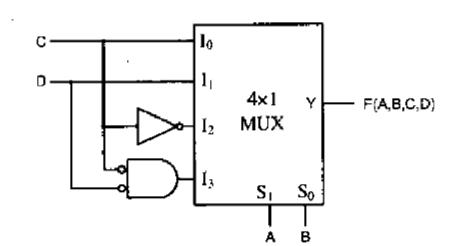
\includegraphics[width=0.9\textwidth]{esp 32.png} % Change filename if needed
\end{center}

\vspace{1em}

\noindent\textbf{Options:}
\begin{enumerate}[label=\textbf{\Alph*.}]
  \item P–2, Q–4, R–1, S–3
  \item P–4, Q–2, R–1, S–3
  \item P–2, Q–4, R–3, S–1
  \item P–4, Q–2, R–3, S–1
\end{enumerate}

\vspace{1em}
\section*{\textcolor{blue}{Explanation}}

\begin{itemize}
  \item \textbf{P:} The symbol in P is a \textbf{NOR gate}, which is the negation of OR. Its match in Column B is option 2.
  \item \textbf{Q:} The symbol in Q is a \textbf{NAND gate}, which is the negation of AND. Its match in Column B is option 4.
  \item \textbf{R:} The symbol in R is a \textbf{basic OR gate}. Its equivalent is option 1.
  \item \textbf{S:} The symbol in S is a \textbf{basic AND gate}. Its match is option 3.
\end{itemize}

\noindent Therefore, the correct matching is:
\[
\boxed{
\text{P–2,\quad Q–4,\quad R–1,\quad S–3}
}
\]
\vspace{1em}
\noindent\textbf{Correct Answer:} \fbox{(A) P–2, Q–4, R–1, S–3}

\end{document}
